\chapter{Pulse Generation by XFEL}
Free-electron lasers (XFELs), invented by J. Madey and demonstrated experimentally in the 1970s, can generate multi gigawatt and femtosecond (fs) x-ray radiation. Compared to fourth generation synchrotrons, this is a ten billion-time increase in brightness. Typically an XFEL consists of three sections: i) the electron gun, ii) a linear accelerator, and iii) an undulator. The x-ray radiation is generated in the undulator. Figure 1 shows a schematic of the XFEL at the Linear Accelerator Coherent Light Source (LCLS) at Stanford. This chapter will describe the operating of the LCLS in specific. Other XFELs might use different hardware, but the fundamental principles that drive an XFEL will be very similar. Please note that the words bunch and pulse are used to discriminate between a collection of electrons and radiation respectively.

\begin{figure}[h]\label{fig:LCLS}
\centering
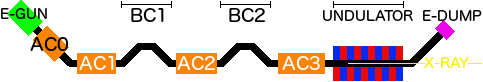
\includegraphics[width=100mm]{LCLS_schematic.png}
\caption{Schematic of LCLS. Electron bunches are created by the electron gun (E-gun). The bunches are consecutively accellerated by linear accelerators (AC0-3) and compressed by bunchcompressors (BC0-1). After the final acceleration the bunch is guided into the undulator, where an x-ray pulse is generated. After the undulator the x-ray pulse continuous to the beamline, and the electron bunch is dumped (E-dump).}
\end{figure}

In the electron gun, a copper plate is irradiated by a powerful ultraviolet laser pulse, which releases a bunch of electrons. At this moment the electron bunch is a few picoseconds long and has a peak current less than 100 A. As shown in figure \ref{fig:AC}a, the energy spread within the bunch is minimal at this point. The electron bunch is directly accelerated to 99.7\% of the speed of light, using a standing wave in a RF cavity (AC0). Due to cooling reasons in AC0 the LCLS produces electron pulses at maximally 120 Hz. 

\section{Klystron}

Consecutively the bunches are guided in a long series of accellerating units named klystrons. See AC1-3 in figure \ref{fig:LCLS}, and for more detail figure\ref{fig:AC})d. In essence a klystron is a cylinder on which an strong MHz alternating current is applied. The AC current induces a EM field in the MHz range (RF), similar to the way radiowaves are produced in an antenna. Due to the spacing between irises the relative phase velocity of the wave is matched to the speed of the electrons, thus through the Lorentz force longitunal acceleration can be achieved throughout the whole klystron. In the center of the cavity the magnetic field is zero, the acceleration is therefore proportional to the strength of the electric field. Each klystron can maximally add 30 MW/m of energy to the electron bunch. Under higher currents the klystron will tear itself apart. In order to reach 15 GeV electron bunches at least 500 m of klystrons are needed. In reality the accelerating unit of LCLS are 889 m long. Often accelerators do not operate at the point of maximum acceleration, since one wants to introduce a negative energy gradient along the particle bunch, that can later be utilized for bunch compression. This acceleration method is called off-crest acceleration, and is visualized in figure  \ref{fig:AC} b and d. A negative energy gradient means that the electrons located at the front of the bunch have a slightly lower energy compered to electrons the electrons are located at the rear of the bunch.

\begin{figure}[h]\label{fig:AC}
\centering
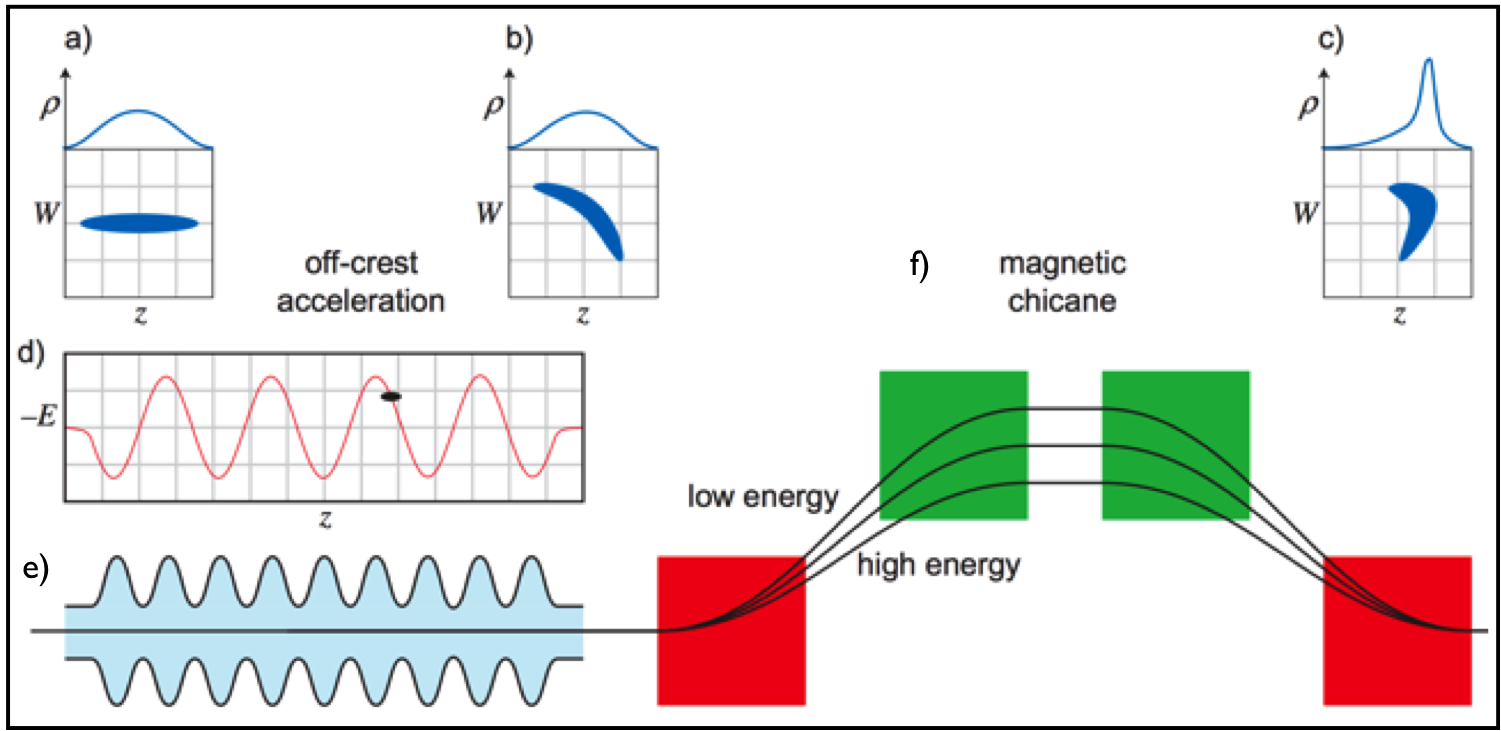
\includegraphics[width=100mm]{acceleration.png}
\caption{Schematic of Acceleration and bunch compression at LCLS. a-c) change of bunch shape throughout the accelerator. d) illustration of the off-crest accelleration principle. a) shows that  This creates an energy chirp. e) schematic of a single klystron. f) schematic of a chicane. The green and red blocks are magnetic dipoles that deflect the electron bunch in opposite direction. The path of high energy electrons diverges less than lower energy electrons. If the bunch has a negative energy chirp, this results in bunch compression.}
\end{figure}

\section{Bunch Compression}
Short and compact bunches are essential for the functioning of an XFEL. One of the main bunch-compression devices are chicanes. Chicanes consist of four magnetic dipoles that diverge the high energy part of the bunch less than the low energy part (see figure \ref{fig:AC} ). Due to the negative energy gradient it thus reduces the temporal spread of the bunch. After the final compression the electron bunch is ~40fs long, has a peak current of 4.3 kA, and travels at 99.999\% of the speed of light. The relastivistic $\gamma \sim 2000$. Creating these type of bunches is a noteworthy technical achievement, 

\section{Undulator}
\subsection{Monochromatic X-ray radiation}
The undulator is the heart of an XFEL. It is a periodic arrangement of magnets with alternating poles. The magnetic field of a periodic magnetic structure can be written as:
\begin{equation}\vec{B}(z) = B_0\cos{(\frac{2\pi}{\lambda_u}z)}\hat{\mathbf{y}}\label{eq:bz}\end{equation}
$B_0$ is the magnetic field, $\lambda_u$ is the wavelength of an undulator period.
Due to the magnetic field the moving bunch of electrons experience a Lorentz force, causing it to oscillate in the transverse direction (x). The movement can be described by the following equation. 
%\begin{equation}\vec{F} = e(\vec{v}\times\vec{B})\end{equation}
\begin{equation}v_x = \frac{-e\,B_0\,\lambda_u}{2\pi\,m_e\gamma} \sin{(\frac{2\pi}{\lambda_u}z)} = \frac{K c}{\gamma} \sin{(k_uz)}\label{eq:vx}\end{equation}
Usually the non-dimensional parameter K is written as:
\[K =  \frac{-e\,B_0\,\lambda_u}{2\pi\,m_e \, c}  \approx 0.9337 B_0 \lambda_u\]
where the magnetic field is measured in Tesla and the undulator period in centimeters.

Preserving momentum the oscillating electrons emit radiation ($\lambda_s$). As described in chapter 1, interference effects will occur between the emitted waves from the different charges (remember the electrons come in a bunch which has a size). The essence of this interference phenomenon lies in the longer route taken  by the oscillating electrons compared to the radiation, which causes an OPD between the radiation emitted by electrons one undulator period apart. If the OPD between the electrons and the radiation is equal to and integer of $\lambda_s$, the emitted waves will add coherently. Radiation with other wavelengths will interfere destructively. The longer an undulator the more pronounced the selection of specific wavelengths. Equation \ref{eq:res} describes this so-called resonance condition.%, as shown in figure 3b.
\begin{equation}c\frac{\lambda_u}{<v_z>} -\lambda_u\, \cos{(\theta)} = n \lambda_s \label{eq:res}\end{equation}
To predict at which wavelength this happens we need to find the average longitudinal velocity $v_z$. As the total speed $v$ of the electrons is not affected by the Lorentz force, $v_z = \sqrt{ {v}^2-{v_x}^2}$\footnote{Using Pythagoras' theorem}. Using Equation \ref{eq:vx} for $v_x$ and $\gamma^2 \equiv (1-\frac{v^2}{c^2})^{-1}$, we can write $v_z$ as: 
\[ v_z = \sqrt{c^2(1-\frac{1}{\gamma^2})-\frac{K^2 c^2}{\gamma^2}\sin^2(k_u\,z)} = c \sqrt{1-\frac{1}{\gamma^2}(1-K^2\sin^2(k_u\,z))}\]
Using the mathematical identity $\frac{1}{\pi}\int_{0}^{\pi} \sin^2( x ) \, dx =\frac{1}{2} $, integrating of half a undulater period gives the average velocity $<v_z>$.
\[<v_z> = c\sqrt{1-\frac{1}{\gamma^2}(1-\frac{K^2}{2})}\]
${\gamma} \gg 1$, thus we can expand the root $\sqrt{1+x} = 1+\frac{1}{2}x-\frac{1}{8}x^2+ ...$ (first order Taylor expansion).
\[<v_z> \approx c(1-\frac{1}{2\gamma^2}(1+\frac{K^2}{2}) )\]
If we now assume that we only observe the radiation in the forward direction, we can expand $\cos{(\theta)} = 1-\frac{\theta^2}{2}$. 
Equation \ref{eq:res} can thus be written as:
\[ n \lambda_s = \lambda_u[\frac{1}{1-\frac{1}{2 \gamma^2}(1+\frac{K^2}{2})} - (1-\frac{\theta^2}{2})]\]
The geometrical series $\frac{1}{1-x} = 1+x+x^2+...$ allows us to obtain the well known undulator equation.
\begin{equation} n \lambda_s = \frac{\lambda_u}{2 \gamma^2}(1+\frac{K^2}{2}+(\gamma\theta)^2)\end{equation} 

This formula can be explained by two relativistic effects. For an observer it is the electron bunch that is moving close to the speed of light. In the electron bunch's frame of reference however it is the undulator that is moving very fast. Fast objects are length contracted, thus the electrons observes a undulator period of $\frac{\lambda_u}{\gamma}$, which makes it emit radiation with $\lambda$ around $\frac{c\lambda_u}{\gamma}$. The radiation is relativistically contracted when observed in the laboratory's frame of reference (relativistic doppler effect), adding the second gamma term. The size of relativistic doppler effect is dependent on the angle of observation relative to the direction of motion. 

The final wavelength of the emitted light is thus dependent on the energy of the electrons ($v$), the magnetic field in the undulator ($B$), and the angle of observation ($\theta$). Control over these variables makes the selection of a specific wavelength possible. LCLS can produce X-ray radiation in the range of 400 eV -10 keV. 


%\subsection{Direction of Emission}
\subsection{SASE}
So far the emitted radiation is monochromatic, but not temporally coherent. This means the total emitted power is proportional to the number of the electrons in the bunch ($N_e$). If all emitted radiation would emit in phase, the total irradiated power would be proportional to ${N_e}^2$. Pellegrini and others realized that for short pulses, and long undulators, temporal coherence could by achieved by a process called Self Amplified Stimulated Emission (SASE). SASE exploit the slight non-uniformities in the electron bunch, that cause radiation with a certain phase to be slightly more prevalent than others. The Coulombic force exerted by the electric field of this radiation will start grouping electrons at its nodes (See figure 2). Electrons are accelerated when the electric field is positive, and decelerated when negative, causing the so-called microbunches to appear. This process forms a positive feedback loop, causing a exponential increase in radiation power. The  exponential  growth  cannot  continue  indefinitely, and  the  power  must  saturate  at  a  certain  level. The SASE process ultimately saturates when either the electrons loose so much energy the resonance condition is not met anymore, or when the energy of the radiation surpasses that of the electron bunch. In the latter case the EM wave will start to transfer energy to the electron bunch instead\footnote{This phenomenon is similar to inverse Compton scattering, in which electrons absorb energy from the radiation field.}.

The high power density within the pulse means that there are more than one photon in the volume of a $\lambda^3$. Which means that so far diffraction patterns come from single photons interfering with themselves []. Interference between more than one photon might be different. For example there might be special interactions between photons. 

\section{Improvements}

Seeding
Multi-angle
High rep rate




